\documentclass{article}

% --- load packages ---

\usepackage[margin=1in]{geometry} % change the margins
\usepackage{amsmath} % useful math environments and commands like align
\usepackage[colorlinks,bookmarks,bookmarksnumbered,allcolors=blue]{hyperref} % hyperlinks between references
\usepackage{graphicx}  % include images
\usepackage[caption=false]{subfig} % subfigures.  false option prevents conflicts in caption styling with other packages
\usepackage{booktabs} % better tables
\usepackage[capitalise]{cleveref} % better referencing. uses cref.
\usepackage[section]{placeins} % sometimes useful to prevent figures from floating out of a section
\usepackage{cite} % handles multiple citations in one command better
\usepackage{doi} % allow correct hypderlinking of DOIs



\begin{document}

\title{Homework 1}
\author{Jaron Ellingson}
% put in \date{} if you don't want a date to appear, or enter a specific date, otherwise default is today's date.
\maketitle

\section*{Abstract}

The following describes two optimization problems, one unconstrained and one constrained. The homework assignment explores using a optimization solver using python. It also explores topics such as dimensionality and accuracy trade offs.

\section{Brachistrochrone}

\subsection{Introduction}

\begin{equation}
\begin{aligned}
\text{minimize} & \quad J=\sum_{i=1}^{n-1} \frac{\sqrt{\Delta x_i^2+\Delta y_i^2}}{\sqrt{H-y_{i+1}-\mu_{k}x_{i+1}} + \sqrt{H-y_i-\mu_i x_i} } \\
\text{with respect to} & \quad y_1 ... y_{n-1} \\
\text{subject to} & \quad x_0=0, y_0=1, x_n=1, y_n=0  \\
\end{aligned}
\end{equation}

For complete problem formulation and parameters see \cite{ning}.

\subsection{Results}


%\begin{figure}[htbp]
%	\centering
%	\subfloat[first subcaption]{
%		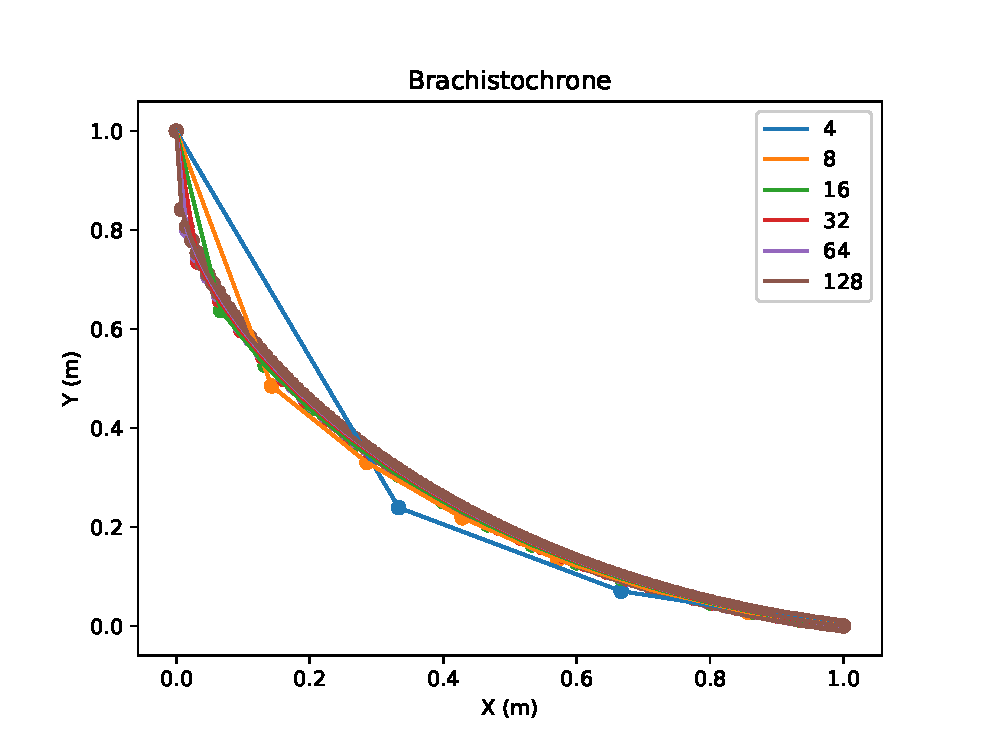
\includegraphics[width=0.45\textwidth]{figures/brachistrochrone.eps}
%		\label{fig:sub1}
%	}
%	\qquad
%	\subfloat[second subcaption]{
%		\includegraphics[width=0.45\textwidth]{figures/128pts.eps}
%		\label{fig:sub2}
%	}
%	\caption{Overall caption, which should be a sentence.}
%	\label{fig:sub}
%\end{figure}

\begin{figure}[htbp]
	\centering
	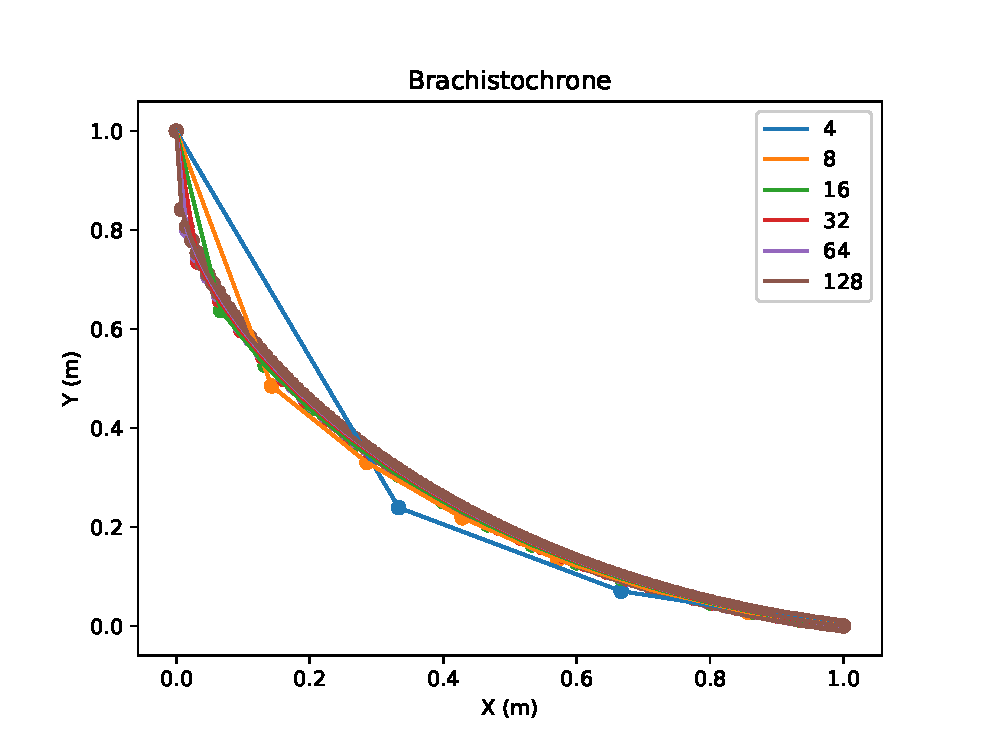
\includegraphics[width=0.75\textwidth]{figures/brachistrochrone.eps}
	\caption{Overall caption, which should be a sentence.}
	\label{fig:results}
\end{figure}

\begin{figure}[htbp]
	\centering
	\includegraphics[width=0.75\textwidth]{figures/dimensionality.eps}
	\caption{Overall caption, which should be a sentence.}
	\label{fig:dimensionality}
\end{figure}


\section{Truss}

\begin{figure}[htbp]
	\centering
	\includegraphics[width=0.75\textwidth]{figures/truss.eps}
	\caption{Overall caption, which should be a sentence.}
	\label{fig:truss}
\end{figure}


\begin{table}[htb]
	\centering
	\caption{This is a table caption.  Note that table captions go above tables, whereas figure captions go below figures.}
	\label{tab:mytable}
	\begin{tabular}{c|c|c}
		\toprule
		Member & Cross-Sectional Area (m$^2$)& Stress (psi) \\
		\midrule
		1 & 7.9 & 25e3 \\
		2 & 0.1 & 25e3 \\
		3 & 8.1 & -25e3 \\
		4 & 3.9 & -25e3 \\
		5 & 0.1 & 0 \\
		6 & 0.1 & 25e3 \\
		7 & 5.79827561 & 25e3 \\
		8 & 5.51543289 & -25e3\\
		9 & 3.67695526 & 37.5e3 \\
		10 & 0.14142136 & -25e3 \\
		\bottomrule
	\end{tabular}
\end{table}

% This is for the bibliography.  Note that it is using sample.bib 
% you would need to provide your own bibtex file.

\bibliographystyle{unsrt}
\bibliography{sample}

\end{document}